\utilchap{smokediff - A utility for comparing two FDS cases}
\label{ch:smokediff}
The utility Smokediff compares two FDS cases with the same
geometry.  Smokediff examines two {\tt .smv}\ files looking for
boundary, slice and Plot3D files containing the same type of data
and located in the same region in space. Data in one file is subtracted from corresponding data in the
other.  Smokediff then generates a new {\tt .smv}\ file referencing the differenced boundary,
slice and Plot3D data files. To compare two .smv files named {\tt
casename1.smv}\ and {\tt casename2.smv}\ one would use the command

\begin{lstlisting}
smokediff -smv casename1 casename2
\end{lstlisting}

\noindent The {\tt -smv}\ option caused Smokeview to open after the differencing is complete to examine the differenced results.
Smokediff allows the grid for slice files in casename2 to be
refined by an integer multiple.  Other usage options for Smokediff are
detailed below

\lstinputlisting{SCRIPT_FIGURES/smokediff.help}

\begin{figure}[bph]
\begin{center}
\begin{tabular}{ccc}
\includegraphics[height=\figheightAbar]{SCRIPT_FIGURES/thouse5_slice_diff_005}&
\includegraphics[height=\figheightAbar]{SCRIPT_FIGURES/thouse5_slice_diff_010}\\
5.0 s&10.0 s\\
\includegraphics[height=\figheightAbar]{SCRIPT_FIGURES/thouse5_slice_diff_030}&
\includegraphics[height=\figheightAbar]{SCRIPT_FIGURES/thouse5_slice_diff_060}\\
30.0 s&60.0 s
&\raisebox{0.0ex}[0pt]{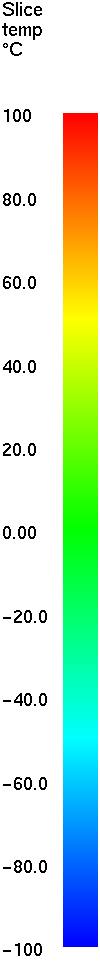
\includegraphics[height=5.5in]{\SMVfigdir/colorbar_m100_100}}\\
\end{tabular}
\end{center}
\caption
[Slice file snapshots of differenced temperature data]
{Slice file snapshots of differenced temperature data.}
\label{figdiffslice}%
\end{figure}
